\chapter{Wi-Fi Protected Access (WPA)}
\label{ch:wpa}


\section{WPA Einführung}
Das \gls{wpaLabel} Protokoll wurde als notwendiger Nachfolger des \gls{wepLabel} Protokolls definiert.
Auch war der weiterführender, sehr umfangreichen Standard \textit{\gls{ieeeLabel} 802.11i} in Arbeit, war aber zum Zeitpunkt als \gls{wepLabel} geknackt wurde noch nicht abgeschlossen. So wurde Anfangs 2003 die ersten zertifizierten \gls{wpaLabel}-fähigen \gls{wlanLabel}-Geräte auf den Markt gebracht.
Seit September 2004 gibt es zertifizierte \gls{wpa2Label} Netzwerkgeräte. Der \gls{wpa2Label} entspricht nun dem \textit{\gls{ieeeLabel} 802.11i} Standard.\footcite{Wi-Fi_Protected_Access__Wikipedia_2015-04-10}\footcite{WPA2__Wikipedia_2015-04-10}
\gls{wpaLabel} nutzt \gls{tkipLabel} zur Verschlüsselung, während \gls{wpa2Label} \gls{aesLabel} verwendet.

\subsection{Sicherheit}
Der \gls{wpa2Label} Standard gilt bis heute als sicher und sollte als einziger Standard verwendet werden.

Da \gls{wpaLabel} und \gls{wpa2Label} sehr viele Ähnlichkeiten aufweisen, wird folgend der Begriff \gls{wpaLabel} übergreifend für beide Standards verwendet. Bei Differenzen wird die jeweilige Version explizit genannt.

Ein erfolgreicher Angriff muss via Bruteforce und Wörterbuch Angriff geschehen, was relativ unmöglich ist, vorausgesetzt es wird ein sicherer \gls{pskLabel} verwendet (mind. 16 zufälligen alphanumerischen Zeichen).

Die ganze Sicherheit basiert auf dem \gls{pskLabel}.
Sobald der bekannt ist, kann eine Verbindung vollständig abgehört werden.
Sprich trotz einem sicherem Schlüssel, kann jeder Netzteilnehmer aktive Verbindungen der anderen abhören, insofern die nicht anderswo verschlüsselt werden (z.B. mit \gls{httpsLabel}).


\subsection{Authentifizierungs-Varianten}
\gls{wpaLabel} bietet nebst der \gls{pskLabel} Methode (auch als \textit{\gls{wpaLabel}-Personal} bekannt), auch eine \textit{enterprise} Methode an, bei der ein Authentifizierung-Server jeden Nutzer einzeln authentifiziert und für jede Sitzung einen neuen \gls{pmkLabel} Schlüssel generiert.
Dieses \textit{enterprise} Protokoll wird oft in Firmen angewendet, lohnt sich aber für den privaten Gebrauch nicht, da der Einrichtungsaufwand und Betrieb eines eigenen Servers zu hoch ist.
Deshalb wird in dieser Arbeit auf die \gls{pskLabel} Methode eingegangen.


\subsubsection{WPS Standard}
Der \gls{wpsLabel} Standard entspricht nicht einer eigener Zugriffs Methode, sondern soll das Einrichten von sicheren \gls{pskLabel} beim Client erleichtern.

Dazu gibt es folgende vier Methoden:\footcite{Wi-Fi_Protected_Setup_-_Wikipedia_the_free_encyclopedia_2015-04-10}
\begin{itemize}
	\item \textbf{PIN:} Ein 8-stelliger PIN des einen Gerätes muss auf dem anderen eingegeben werden.
	\item \textbf{Push button:} Per Kopfdruck am \gls{apLabel} wird eine zweiminütige Beitrittsphase des Netzwerkes gestartet.
	\item \textbf{\gls{nfcLabel}:} Die Daten werden via \gls{nfcLabel} ausgetauscht (was nur innerhalb kurzer Distanz möglich ist).
	\item \textbf{\gls{usbLabel}:} Die Netzinformationen werden via externen \gls{usbLabel} Storage ausgetauscht.
\end{itemize}

Die PIN Methode gilt als besonders unsicher, da lediglich eine 7-stellige Zahl erraten werden muss (die letzte entfällt, da sie einer Checksumme entspricht).
Als Gegenmassnahme kann eine automatische zeitliche Sperre nach fehlgeschlagenen Versuchen eingestellt werden.\footcite{viehboeck_wps_2015-04-10}

\textit{Push button} und \textit{\gls{nfcLabel}} sind anfällig auf ungewollte Nutzer, wenn der \gls{apLabel} an einem unbewachten Ort steht und sich so jemand selbst authentifizieren kann.


\subsection{Schlüsselaustausch}
Voraussetzung für den gewöhnlichen Schlüsselaustausch ist der Besitz des \gls{pskLabel} (entspricht dem \textit{passphrase}).
Dieser Schlüssel kann aus 8 bis 63 druckbaren \gls{asciiLabel} Zeichen bestehen.

\subsubsection{Four-Way Handshake}
%\begin{wrapfigure}{r}{0.5\textwidth}
%	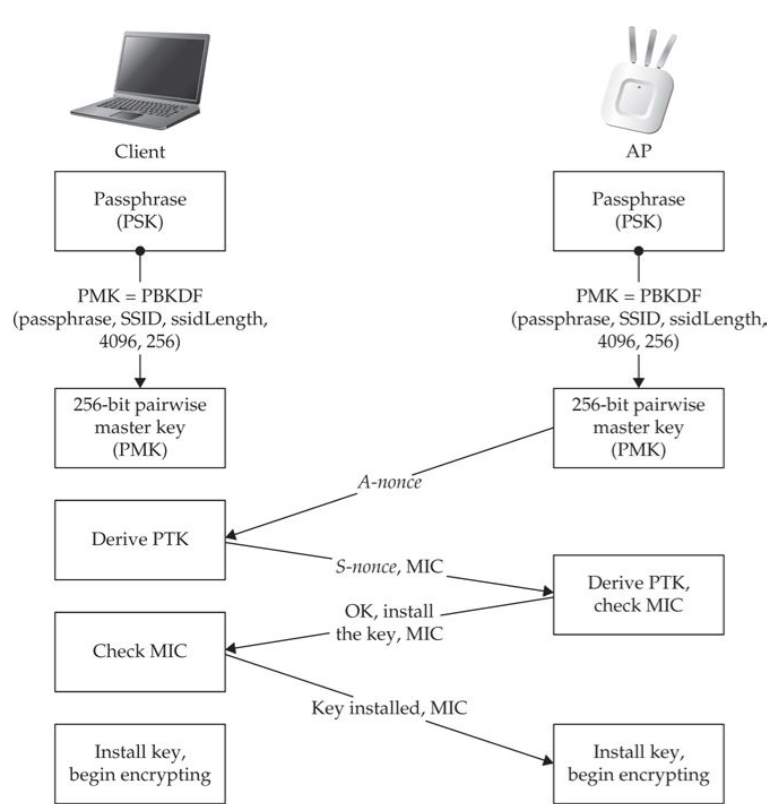
\includegraphics[width=1.0\linewidth]{images/wpa/four-way-handshake.png}
%	\caption[WPA: The four-way handshake]{WPA: \textit{The four-way handshake} (Quelle: \cite[][151]{WrightCache201503})}
%\end{wrapfigure}
\begin{figure}[H]
	\centering
	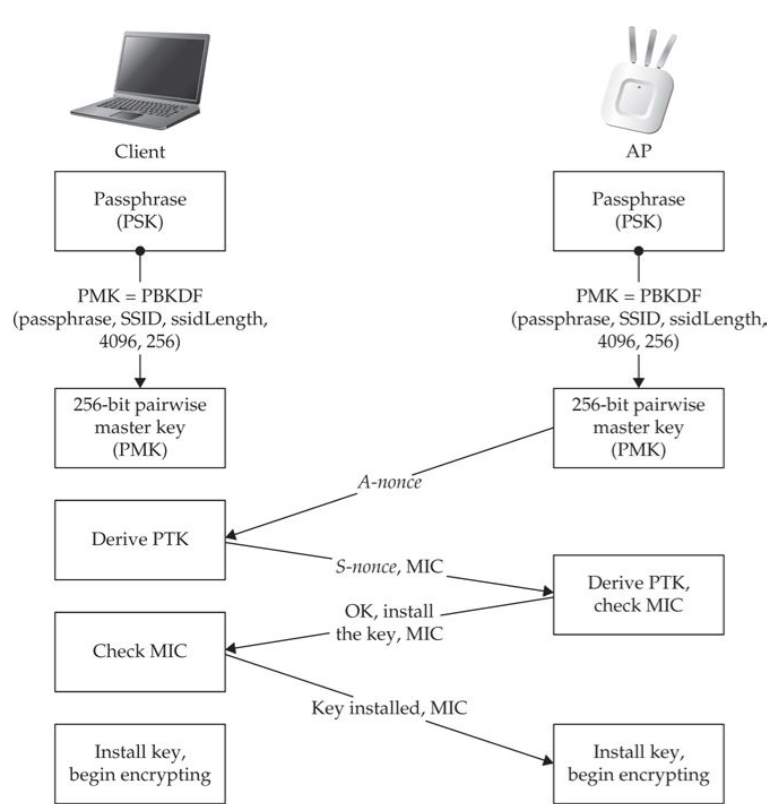
\includegraphics[width=0.8\linewidth]{images/wpa/four-way-handshake.png}
	\caption[WPA: The four-way handshake]{WPA: \textit{The four-way handshake} (Quelle: \fullcite[][151]{WrightCache201503})}
\end{figure}
Der \textit{Four-Way Handshake} bezeichnet den Zugriff eines Clients auf das Netzwerk.
Bei einer Verbindung zum Netzwerk wird beidseitig aus dem \gls{pskLabel} und der \gls{ssidLabel} der \gls{pmkLabel} berechnet.
Dafür wird 4096 der Hash (HMAC-SHA1) des \gls{pskLabel} berechnet. (Dies macht einen Bruteforce Angriff so aufwändig.)
Der \gls{apLabel} überträgt dem Client eine zufällige Zahl (\textit{A-nonce}), welche der Client mit einer weiteren zufälligen Zahl (\textit{B-nonce}) ergänzt.
Der \gls{apLabel} berechnet aus den zufälligen Zahlen und den beiden \gls{macLabel}-Adressen einen temporären \gls{ptkLabel}, der pro Session neu generiert wird. Der \gls{ptkLabel} wird zudem auch während einer Session periodisch ausgetauscht.\footcite[][40f.]{WrightCache201503}

%\begin{figure}[H]
%	\centering
%	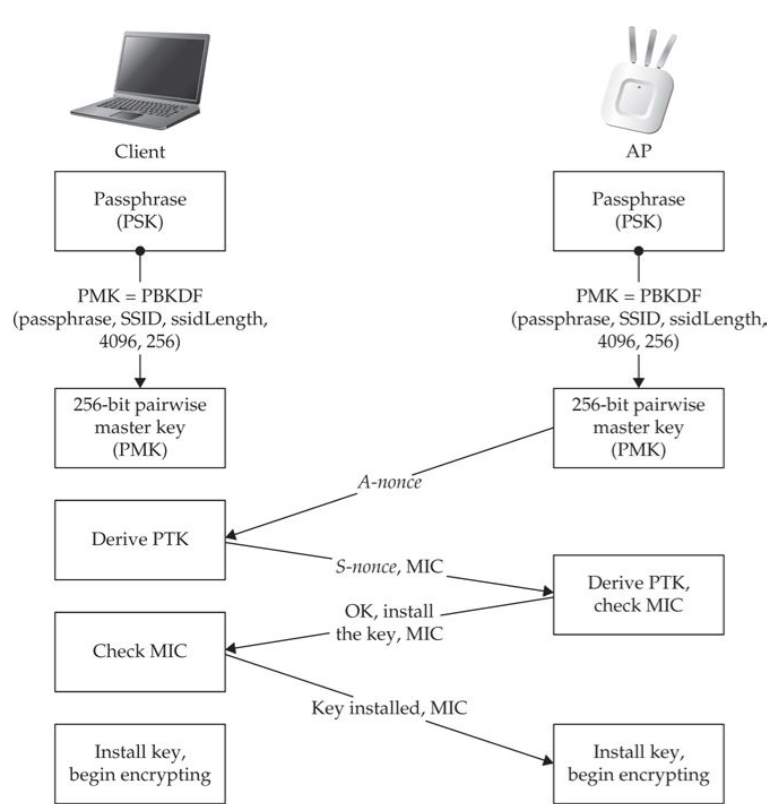
\includegraphics[width=0.6\linewidth]{images/wpa/four-way-handshake.png}
%	\caption[WPA: The four-way handshake]{WPA: \textit{The four-way handshake} (Quelle: \fullcite[][151]{WrightCache201503})}
%\end{figure}

Um den Schlüssel zu knacken werden zusammengefasst folgende Informationen gebraucht:
\begin{itemize}
	\item Netzwerk \gls{ssidLabel}
	\item \textit{A-nonce}
	\item \textit{B-nonce}
	\item \gls{macLabel}-Adresse des Clients
	\item \gls{macLabel}-Adresse des \gls{apLabel}'s
	\item \gls{micLabel} (entspricht einem Hash der Nutzdaten, um Verfälschung erkennen zu können).
\end{itemize}

Nebst während dem \textit{Four-Way Handshake}, werden diese Information auch regelmässig wiederholt.
So muss nicht zwingend ein vollständiger \textit{Four-Way Handshake} vorliegen.


\section{Angriffe (WPA)}
%p148    \footcite[][148f.]{WrightCache201503}:

\subsection{Angriff Methode}
Für einen erfolgreichen Angriff muss ein \textit{Four-Way Handshake} vorliegen.
Dazu müssen die Aktivitäten eines Channel wie in \cref{subsec:wep_crack_tutorial} abgehört und gespeichert werden (z.B. mit \textit{airtport}).
Während der Aufzeichnung, müssen mindestens 2 Teile des \textit{Four-Way Handshake} aufgezeichnet werden.

Falls sich keine Clients neu anmelden, können bestehende Clients rausgeschmissen werden
\begin{lstlisting}[style=lstStyleFramed]
aireplay-ng --deauth 1 -a A4:52:6F:8A:9F:01 -c 2c:f0:ee:20:7c:32 en0
\end{lstlisting}
\begin{tabular}{l l}
	\textbf{Parameter} & \textbf{Bedeutung}
	--deauth 1 & 64 packages to deauthenticate\\
	-a:	& \gls{apLabel} \gls{macLabel}-Address\\
	-c:	& Client \gls{macLabel}-Address\\
	en0 & Interface
\end{tabular}

\subsection{Bruteforce}
\todo{Bruteforce to glossary}
Der Rest des Angriffs kann offline erfolgen. Durch Ausprobieren wird nach einem gültigen \gls{pskLabel} gesucht, der einen gültigen \gls{micLabel}-Hash berechnet. Dies wird für alle Keys durchprobiert.
Es gibt verschiedene Programme die den Bruteforce durchführen können.
Einige davon sind im \cref{subsec:wpa_attack_tutorial} dokumentiert.

\todo{glossary: onpremise von cloud übernehmen}
Die Berechnung ist je nach Schlüssellänge sehr intensiv und wird daher oft statt von der \gls{cpuLabel}, von der \gls{gpuLabel} ausgerechnet.
Zudem kann Berechnung anstatt von einem \textit{\gls{glos:onPremiseLabel}} Rechner, in der \textit{"`\gls{glos:cloudLabel}"'} berechnet werden.


\subsection{Konkreter Angriff auf ein WPA Netzwerk}
\label{subsec:wpa_attack_tutorial}

\begin{lstlisting}[style=lstStyleFramed]
pyrit -r yhxXXXX.cap -o yhxXXXX_strip.cap strip
\end{lstlisting}

\begin{lstlisting}[style=lstStyleFramed]
aircrack-ng yhxXXXX.cap -w wordlist.txt -b A4:52:6F:8A:9F:01
\end{lstlisting}


\begin{lstlisting}[style=lstStyleFramed]
pyrit -r yhxXXXX_strip.cap -i wordlist.txt -b a4:52:6f:8a:9f:01 attack_passthrough
\end{lstlisting}




% aircrack-ng -J YHX-02427 yhxXXXX_strip.cap


